\subsection{Microcontroller}\label{ssec:mcu-review}

\subsubsection{Microcontroller basic characteristics}\label{sssec:microcontroller-basic-characteristics}

A microcontroller is a compact computer on a single integrated circuit chip, in most cases a microcontroller (also refered by the acronym MCU) includes a processor, volatile and non-volatile memory, input/output ports and other peripherals. The great thing about the microcontrollers is their low cost, many small appliances that does not require a powerful hardware are only economically viable because of those devices. The components a microcontroller has may vary, it is a responsability of the project designer to decide the microcontroller that has the best fit (technically and economically) for the project.
	\par
	Microcontrollers differ from microprocessors only in one thing, MCUs can be used standalone while microprocessors need other peripherals to be used. By reducing the size and cost compared to a design that uses a separate microprocessor, memory, and input/output devices, microcontrollers make it economical to digitally control even more devices and processes. \say{A microprocessor can be considered the heart of a computer system, whereas a microcontroller can be considered the heart of an embedded system}\cite{mcuDef}.
	\par
	A great thing about microcontrollers is that they must provide provide real-time response to events, so for instrumentation they are crucial. With them it is possible to acquire signals with good sampling rates without loss of relevant information. It is common in electronic instrumentation to use MCUs to handle the events that have real-time constains and use more sophisticated hardware solutions to manage and process the acquired data later \cite{bartz2004data}.

\subsubsection{Microcontroller ISP programming}\label{sssec:microcontroller-isp-programming}

	In-system programming (ISP), also called in-circuit serial programming (ICSP), is a technique where a programmable device is programmed after the device is placed in a circuit board \cite{icsp-guide} rather than before placing the circuit in the board.
	\par
	There are many different standards protocols for ISP, most of them variants from the Joint Test Action Group (JTAG) protocol \cite{oshana2002introduction}. An example of devices using ISP is the AVR line of micro-controller by Microchip such as the ATmega328PB MCU \cite{atmega328p-datasheet}. According to \cite{equinox-isp}, important ISP definitios are:

	\begin{itemize}
		\item\textit{\textbf{ISP Programmer: }} This is a device which is capable of producing the required logic and power signals to in-system program the \textbf{\textit{Target Microcontroller}}.\label{itm:isp-programmer}
		\item\textit{\textbf{Target Microcontroller: }} This is the MCU which is to be in-system programmed.\label{itm:isp-target-mcu}
		\item\textit{\textbf{Target System: }} The Target System is the physical PCB which contains the MCU to be in-system programmed.\label{itm:isp-target-system}
		\item\textit{\textbf{ISP Header: }} The programmer must interface to the correct pins of the target device, systems that have ISP programmers usually have a standard connector to ensure the connection is done the right way between the programmer and the MCU.\label{itm:isp-header}
	\end{itemize}

	Figure \ref{fig:typical-connections-for-isp-programming} show the typical connection for most AVR ISP systems

		\begin{figure}[htbp]
			\centering
			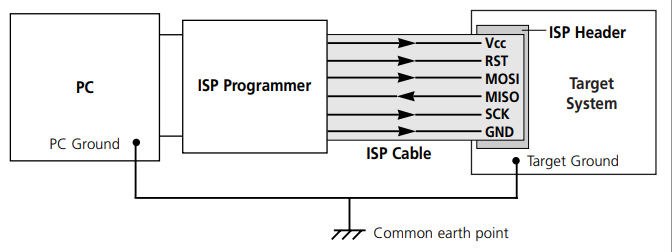
\includegraphics[scale=0.7]{figuras/fig-typical-connections-for-isp-programming.png}
			\caption{Typical Connections for ISP Programming \cite{typical-connections-for-isp-programming}}
			\label{fig:typical-connections-for-isp-programming}
		\end{figure}


	According to \cite{equinox-isp}, the signals from the 6-pin headers are:

	\begin{itemize}
		\item\textit{\textbf{VCC: }} Programmer Vcc Connection.\label{item:isp-vcc}
		\item\textit{\textbf{MOSI: }} Programmer MOSI signal (SPI Data Out).\label{item:isp-mosi}
		\item\textit{\textbf{MISO: }} Programmer MISO signal (SPI Data In).\label{item:isp-miso}
		\item\textit{\textbf{RESET: }} Programmer RESET Control Line.\label{item:isp-reset}
		\item\textit{\textbf{GND: }} Programmer Ground Connection.\label{item:isp-gnd}
		\item\textit{\textbf{SCK: }} Programmer Serial Clock Signal.\label{item:isp-sck}
	\end{itemize}